\chapter{Architectures envisagés}

\section{Préambule}
Le cahier des charges présenté ci-dessus spécifie que l'application doit être
simple et mobile. Malgré certaines recommandations par le client, nous avons
tout de même étudié les choix qui s'offrait à nous en partant de l'existant.

\section{Système OrKestre}

Le système orKestre est un système actuellement sur le marché. Il est aussi
connu sous le nom de système 'Perroquet'.

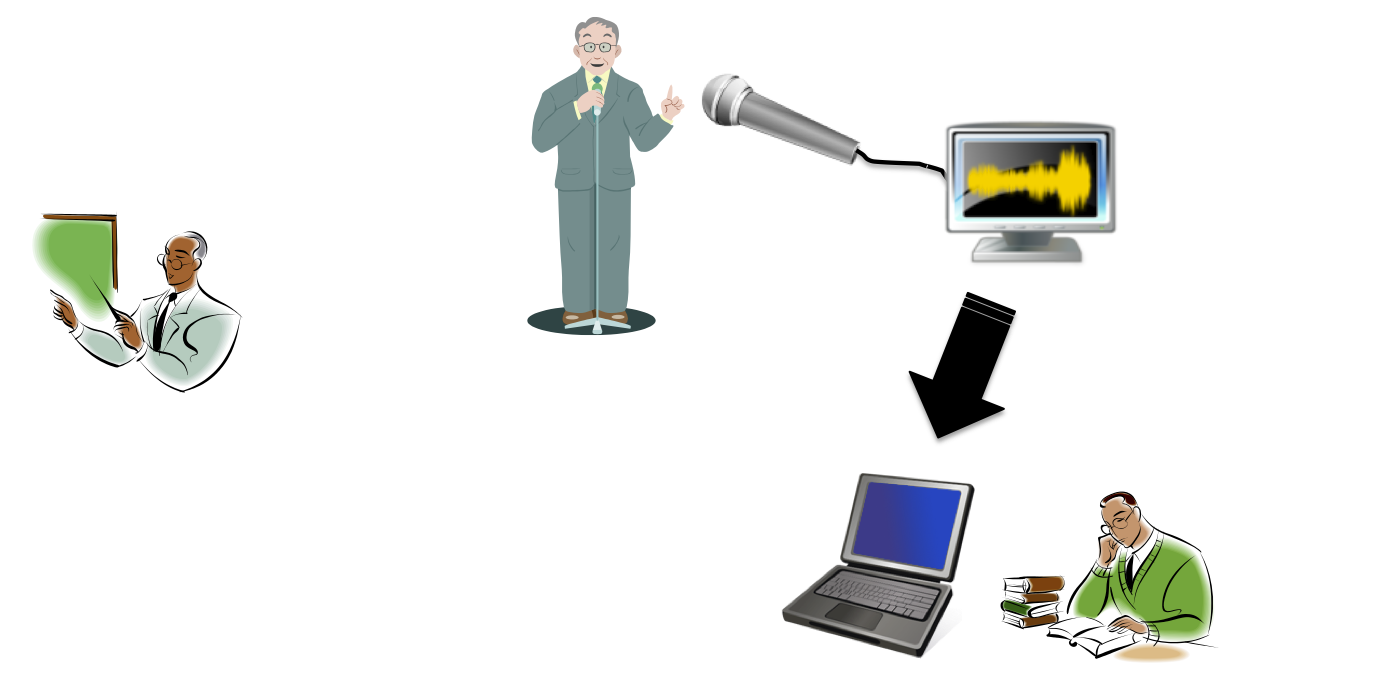
\includegraphics[width=12cm]{img/orKestre.png} 

Il se présente ainsi : Une personne est présente dans le cours et dicte distinctement le cours qu'elle entends du professeur, dans un microphone. Ce microphone est relié à un ordinateur qui dispose d'un moteur de reconnaissance vocale. Une fois le flux audio transformé en texte, ce dernier est envoyé à l'utilisateur malentendant par le réseau wifi ou filaire.

Ce système a pour avantage d'être optimal dans la qualité du texte reconnu par le moteur de reconnaissance vocale. En effet, le dicteur maitrise l'outil et y possède son dictionnaire ainsi que ses modèles vocaux. 
Pour autant, ce système n'est pas utilisable à l'université de Nantes car il nécessite l'engagement d'une personne tierce entièrement consacrée à la diction dans le microphone. Ceci est un problème pour l'université qui ne dispose pas de fond suffisant pour l'emploi et la formation d'une, voire de plusieurs personnes pour ce système.

\section{Solution 1}

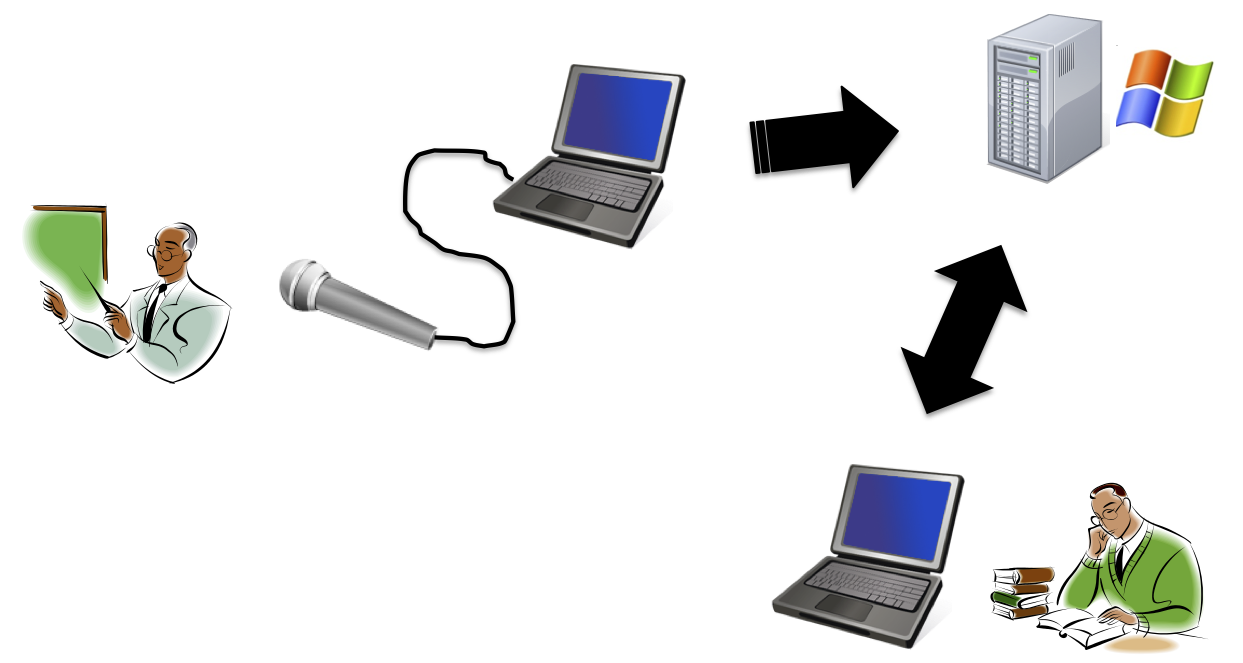
\includegraphics[width=12cm]{img/solution1.png} 

La première solution envisagée suit donc le modèle précédent mais sans une personne tierce. Le microphone est donc directement relié à un ordinateur portable géré par le professeur. Le son est transmit par cette ordinateur à un serveur fonctionnant sous windows XP (requis pour faire tourner speechroot) qui analyse le texte le transmet à un client web sur l'ordinateur de l'utilisateur malentendant.

\subsection{Pour}
Cette solution est la plus simple pour l'utilisateur. En effet, elle ne contraint pas celui-ci à utiliser un système d'exploitation tel que Windows Xp puisque le client web est compatible avec tout système qui fournit un navigateur web. Le texte serait donc affiché sur un site web interne à l'université.

\subsection{Contre}
Le problème est que cette solution n'est pas envisageable car certain professeurs sont réfractaires à l'informatique. Le professeur ne doit donc pas avoir à manipuler un ordinateur mais juste à porter le microphone.


\section{Solution 2}

La solution 2 reprends donc la solution précédente, mais on supprime l'ordinateur manipulé par le professeur.

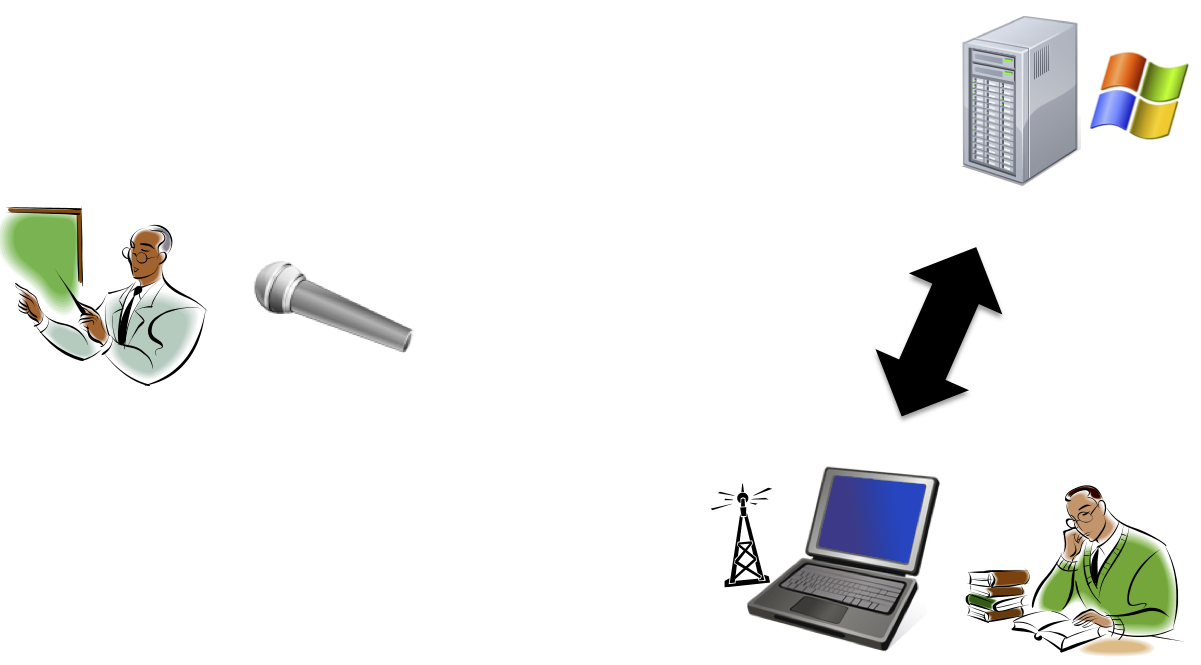
\includegraphics[width=12cm]{img/solution2.png} 


Le microphone perds son fil et est donc un récepteur est connecté à l'ordinateur de l'élève.
C'est donc par son ordinateur que le flux audio est transmis au serveur de l'université qui fait fonctionner le moteur de reconnaissance vocale.

Le texte lui est renvoyé, comme auparavant, dans un client web.

\subsection{pour}
Le professeur n'a pas à se soucier de l'ordinateur portable : l'élève connecte le micro du professeur à son ordinateur personnel.

\subsection{Contre}
Cette solution n'est tout de même pas envisageable à l'université. Bien qu'elle soit la plus simple et la plus mobile pour le professeur et l'elève, l'université refuse de maintenir un serveur fonctionnant sur windows XP.

\section{Solution 3}
La solution 3 est finalement celle que nous avons choisi d'implémenter car c'est la seule qui est réalisable même si on perds en mobilité, utilisabilité et simplicité.

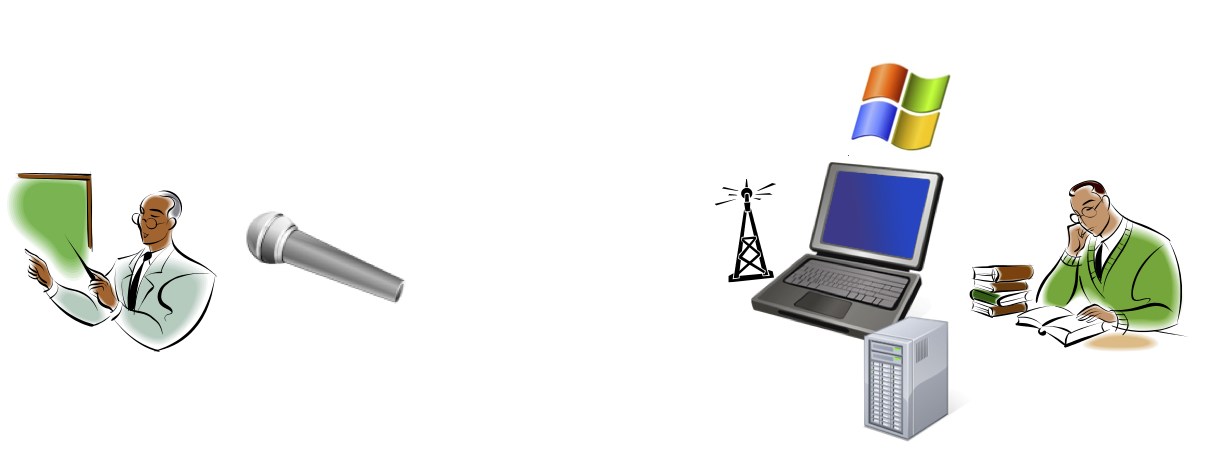
\includegraphics[width=12cm]{img/solution3.png} 

En effet, le moteur de reconnaissance vocale est finalement déplacé sur l'ordinateur personnel de l'étudiant : il est exécuté en tache de fond sur celui-ci. L'ordinateur de l'étudiant exécute donc un logiciel qui est uniquement compatible avec Windows. On perds donc en portabilité mais seule cette solution est réalisable.
